\documentclass{beamer}
% to typeset the presentation as a handout uncomment:
%\documentclass{article}
%\usepackage{beamerarticle}

\usepackage{graphicx,hyperref,url}
\usepackage{color,colortbl}
\usepackage{hyperref}

\newcommand{\myhref}[2]{{\color{blue}\href{#1}{#2}}} 

\usecolortheme{beaver}
\usetheme{Goettingen}

\beamertemplatenavigationsymbolsempty

\usefonttheme[onlymath]{serif}

\makeatletter
\setbeamertemplate{sidebar canvas right}%
                  [vertical shading][top=red,bottom=gray]
\setbeamertemplate{footline}{\hfill\insertframenumber/\inserttotalframenumber}
\makeatother


\title{In-Network Processing for LoRaWAN Enabled Systems}

\author[D. Richert]{Dean Richert \inst{1} \\ \scriptsize{with H. Leung \inst{1}, N. Xie \inst{2}, C. Adderley \inst{2}, and K. Hussein \inst{2}}}

\institute[University of Calgary]
{
  \inst{1} Department of Electrical and Computer Engineering\\
  Schulich School of Engineering\\University of Calgary \\ \vspace{5mm}
  \inst{2} Information Technology, City of Calgary
}

\logo{%
    
\includegraphics[width=2cm,height=2cm,keepaspectratio]{figures/uc_logo.jpg} \hspace*{1cm} {\color{black} November 30, 2017} \hspace*{1cm} 
\includegraphics[width=2cm,height=2cm,keepaspectratio]{figures/schulich.png}
}

\date{\scalebox{1}{\insertlogo}}

%\AtBeginSection[]
%{
%  \begin{frame}<beamer>{Outline}
%    \tableofcontents[currentsection,currentsubsection]
%  \end{frame}
%}

\begin{document}

\begin{frame}
  \titlepage
\end{frame}

\begin{frame}{Outline}
  \tableofcontents
\end{frame}


\section{In-Network Processing}
    
    \begin{frame}{In-Network Processing}
        \begin{itemize}
            \item Bringing the computation to where the data is collected
            \item Motivation: 
            \begin{enumerate}
                \item Efficient use of limited resources (network traffic, power consumption)
                \item Reduce amount of stored data in the data centre
                \item Improved security and privacy
            \end{enumerate}
            \item Other names: in-situ processing, device/sensor-level analytics, edge analytics
            \begin{center}
                \begin{figure}
                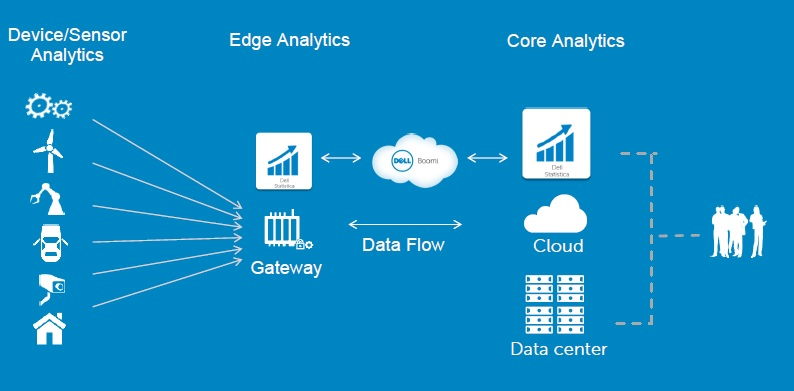
\includegraphics[scale=0.4]{figures/edgeanalyticsarchitecture.jpg}
                \\ \tiny{image adapted from ``Executing on the promise of the Internet of Things (IoT)" by DellWorld}
                \end{figure}
            \end{center}
        \end{itemize}
    \end{frame}
    
    \begin{frame}{In-Network Processing: LoRaWAN}
        Recall that LoRaWAN enables low-power, wide area communication at the expense of bandwidth.
        \vfill
        \begin{center}
            \hspace*{-3mm}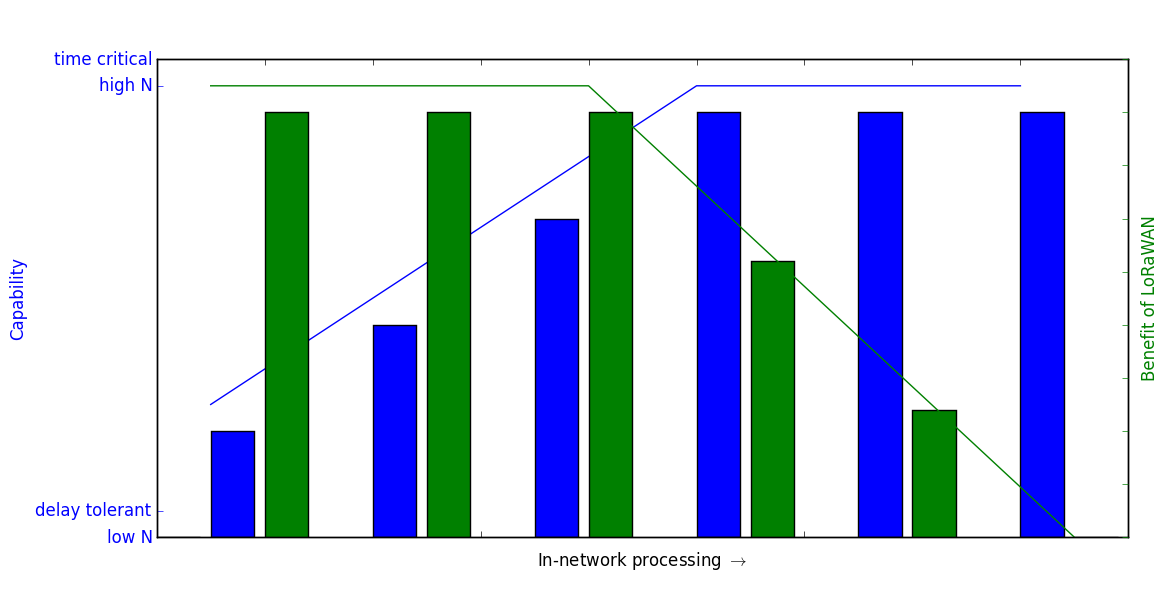
\includegraphics[scale=0.35]{figures/figure_1.png} \\
        \end{center}
        
    \end{frame}

\section{Use cases}
    
    \begin{frame}{Use cases: Event characterization and classification}
        \begin{minipage}{0.6\linewidth}
            {\bf Problem description:} identify to which category a data point/stream belongs to.
        \end{minipage}
        \begin{minipage}{0.35\linewidth}
            \begin{center}
                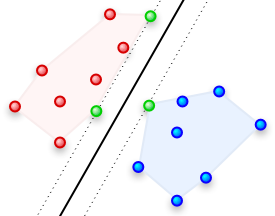
\includegraphics[scale=0.3]{figures/mj-01-svm.png}
            \end{center}
        \end{minipage}
        \vfill 
        {\bf Role of in-network processing:} 
        \begin{itemize}
            \item pre-process a data stream (filtering, dimensionality reduction, etc.)
            \item apply classifier or, more interestingly, train classifier using the new observation (unsupervised learning) 
            \item make data transmission decisions based on result
        \end{itemize}
        \vfill 
        {\bf Examples:} Identifying noise sources, detecting objects in an image 
    \end{frame}
    
    \begin{frame}{Use cases: Training spatially distributed models}
        \vspace*{0cm}
        {\bf Problem description:} train model parameters to predict future events.
        \begin{center}
            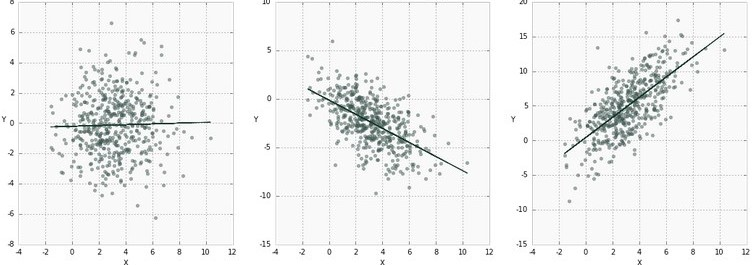
\includegraphics[scale=0.3]{figures/pearson-correlation-3-examples.jpg}
        \end{center}
        \vfill 
        {\bf Role of in-network processing:} 
        \begin{itemize}
            \item pre-process a data stream (filtering, dimensionality reduction, etc.)
            \item refine model parameters using the new observation
            \item incorporate results of neighbouring sensors to enhance the model 
            \item make data transmission decisions based on result
        \end{itemize}
        \vfill 
        {\bf Examples:} weather prediction, crime prediction, predictive maintenance 
    \end{frame}
    
\section{Algorithms}
    
    \begin{frame}{Algorithms: Classical}
        \begin{itemize}
            \item Thresholding
            \item Averaging
            \item Filter banks: Decompose a data stream into multiple frequency bands
            \item Recursive least squares: incorporate new data to refine a linear model
            \item Kalman filtering: track the state of a dynamical system
        \end{itemize}
    \end{frame}
    
     \begin{frame}{Algorithms: State-of-the-art}
        
        Network-enhanced analytics:
        \begin{center}
            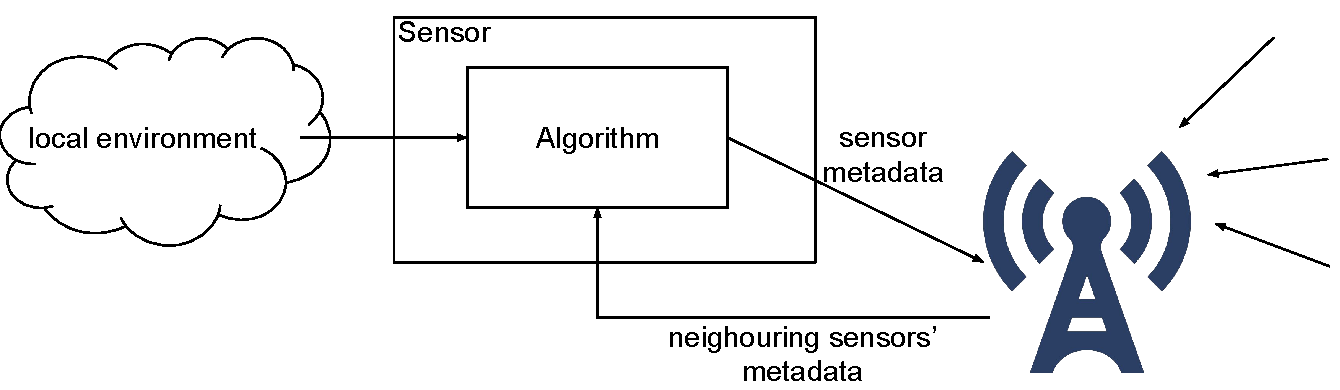
\includegraphics[scale=0.3]{figures/data_fusion.pdf} \\
        \end{center}
        \begin{minipage}{0.5\linewidth}
            \begin{itemize}
                \item clusters naturally emerge, giving insight into underlying phenomema
            \end{itemize} 
        \end{minipage}
        \begin{minipage}{0.45\linewidth}
            \begin{center}
                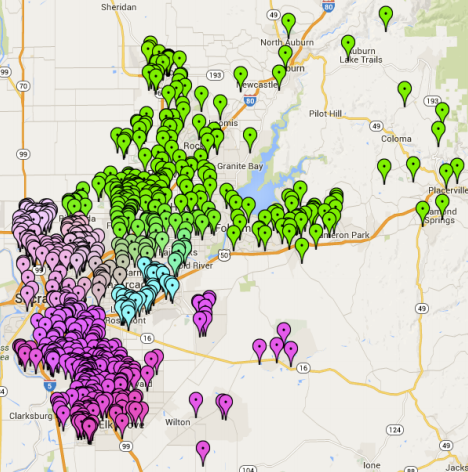
\includegraphics[scale=0.3]{figures/network-enhanced.PNG}
            \end{center} 
        \end{minipage}
    \end{frame}

\section{Hardware considerations}
    
    \begin{frame}{Hardware considerations}
        To fully exploit the benefits of LoRaWAN, your sensor will likely be {\bf battery powered} and {\bf cheap}. Therefore, power consumption balanced with processing power will be your primary consideration.
        \vfill 
        The main hardware components include:
        \begin{itemize}
            \item Microcontroller: respectable computing power with very low current consumption --- a lithium-ion battery can power some MCUs for over {\bf 10 years}!
            \begin{itemize}
                \item Most MCUs include the basic peripherals needed to control the transceiver (SPI, UART) and read digital or analog sensors (I2S,SPI,ADC) 
            \end{itemize}
            \item Transceiver: implementing the LoRaWAN protocol. Typical transmit current consumption is 125mA
            \item Low-power sensor(s)
            \item High-capacity battery: lithium-ion
        \end{itemize}
    \end{frame}
    
\section{CoC/UofC collaboration}
    
    \begin{frame}{CoC/UofC collaboration}
        \vspace*{0cm}
        {\bf Project overview:} Design and deploy $\approx 30$ acoustic sensors to monitor noise levels and characterize noise sources.
        \vfill 
        \begin{minipage}{0.5\linewidth}
            {\bf Current status:} Working prototype has been designed. PCB design is almost complete. Data analysis and visualization toolbox developed.
        \end{minipage}
        \hspace*{2mm}
        \begin{minipage}{0.45\linewidth}
            \begin{center}
                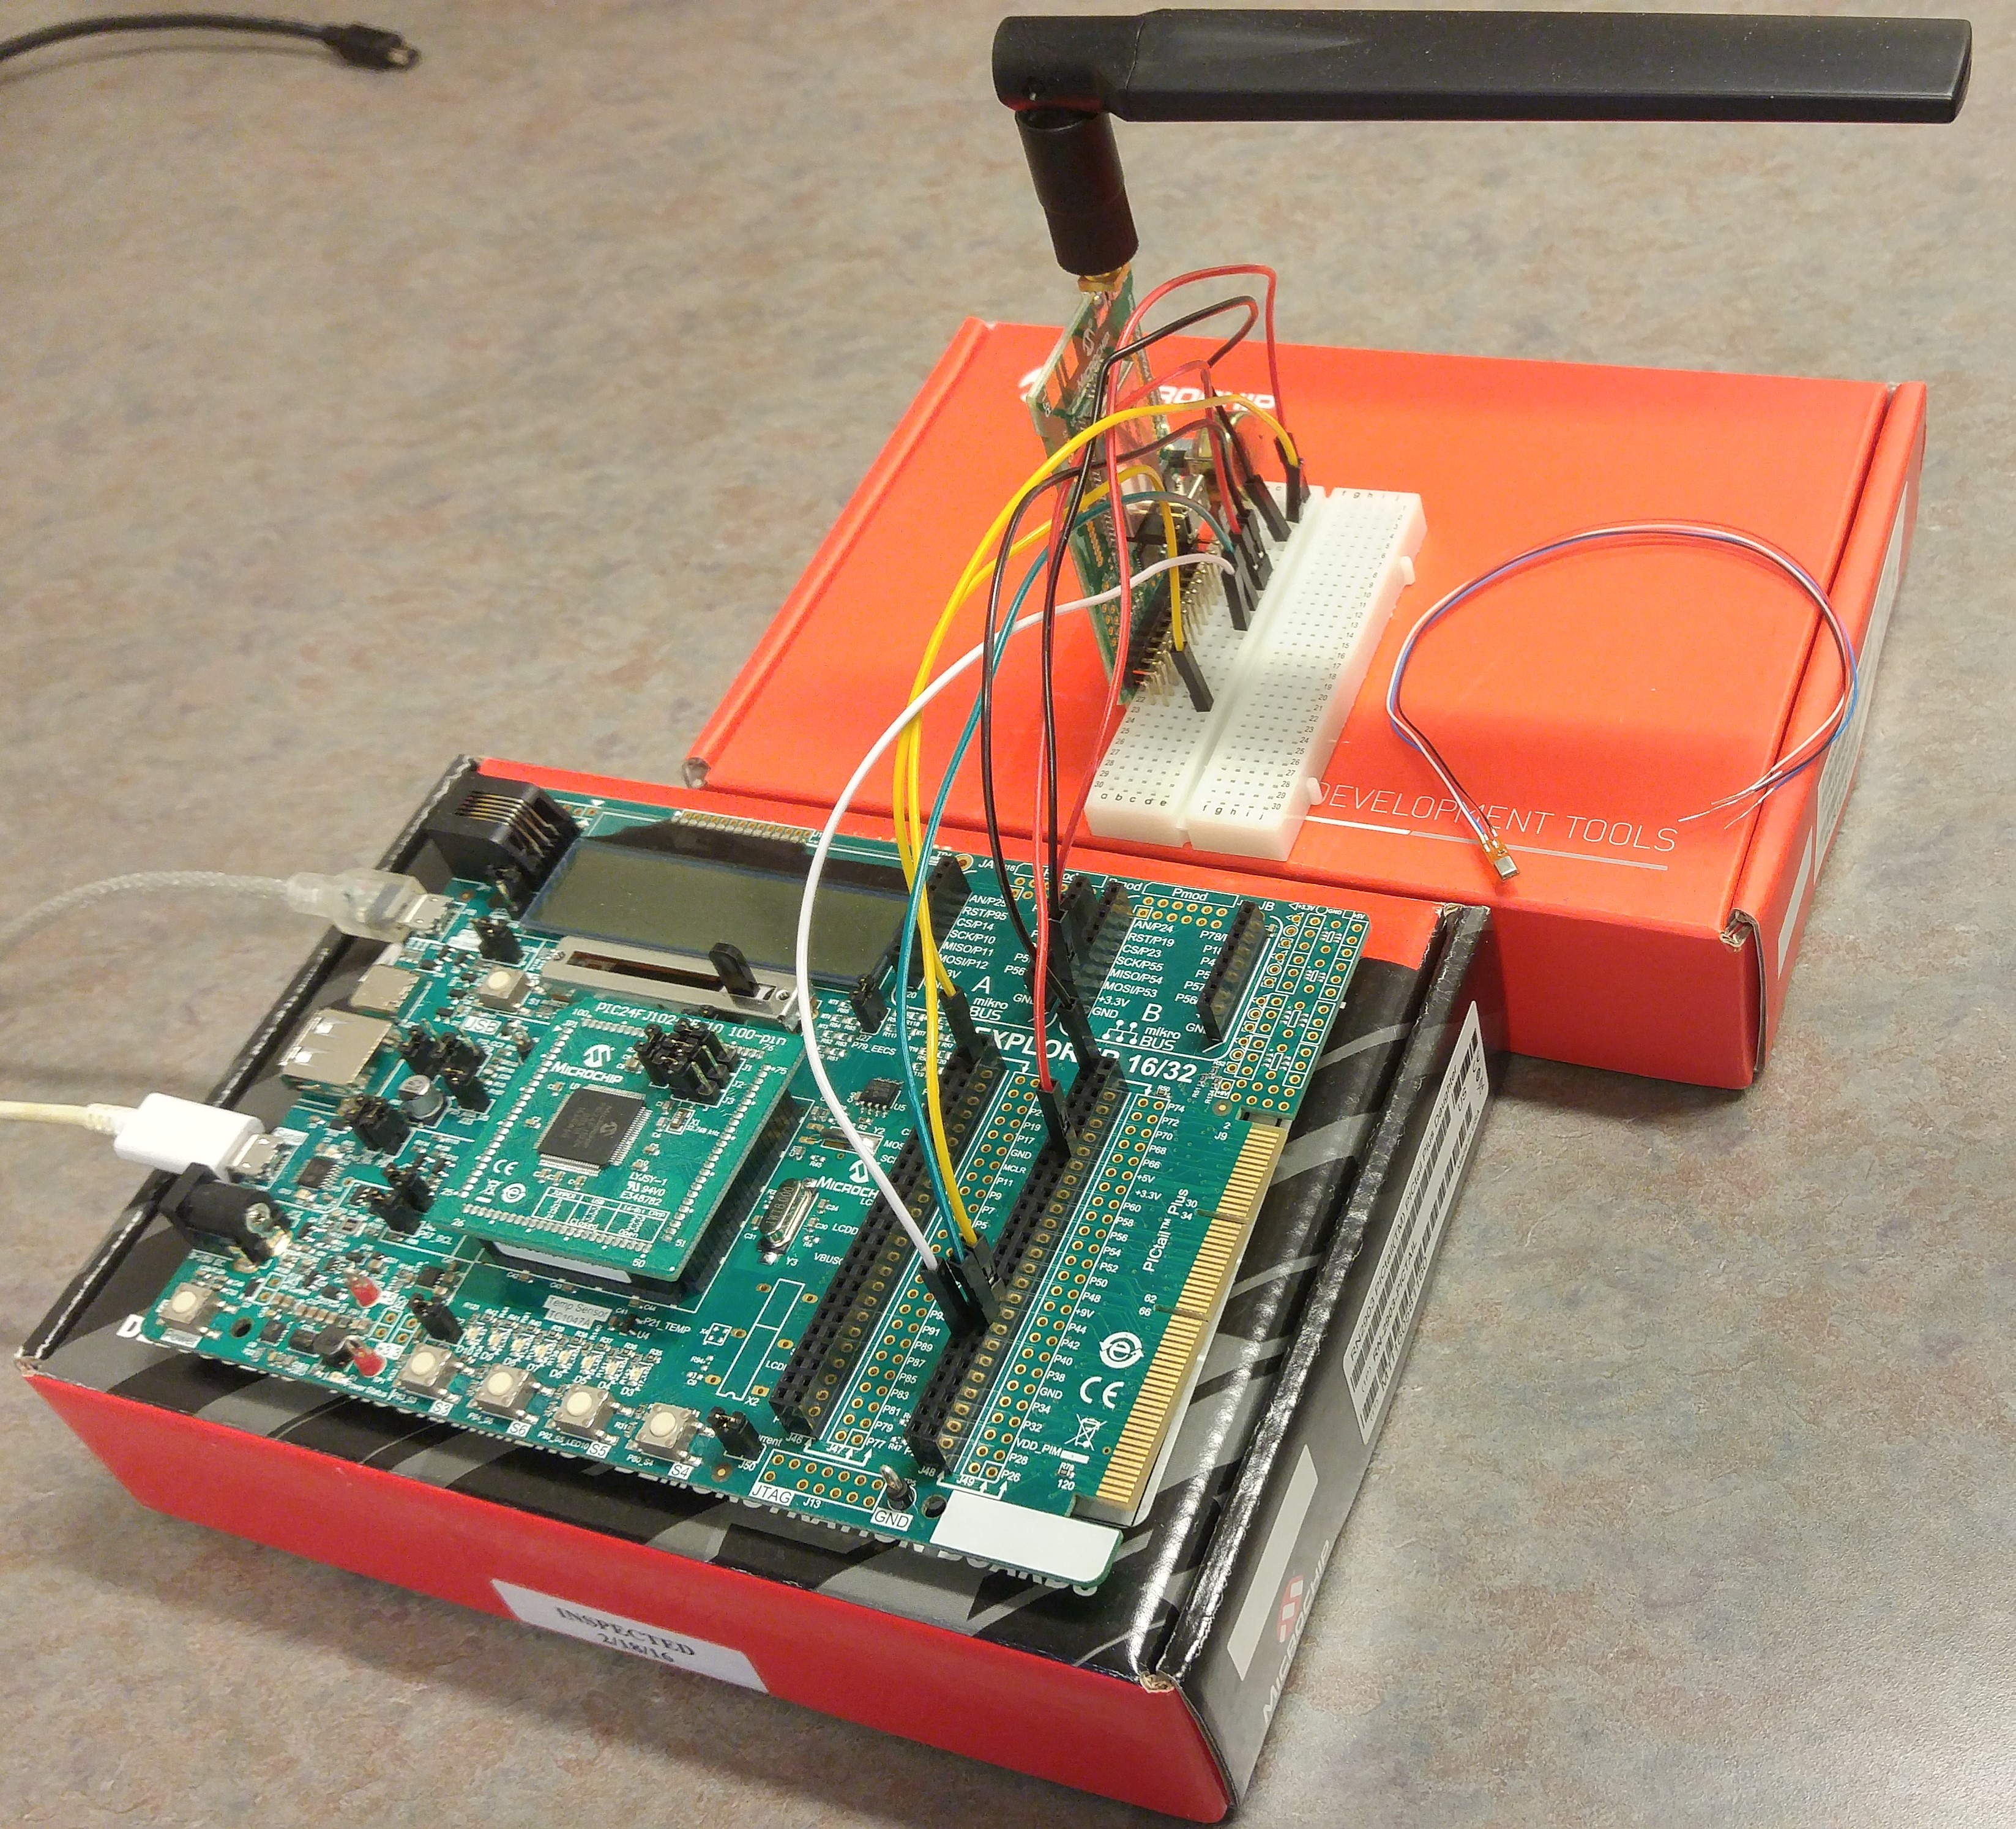
\includegraphics[scale=0.04]{figures/20170927_112827_HDR.jpg}
            \end{center}
        \end{minipage}
        \vfill 
        {\bf Target use cases:} Bylaw enforcement (noise pollution), gunshot detection, spatial/temporal modeling, noise reduction. 
    \end{frame}
    
\end{document}
